\documentclass[11pt, a4paper]{article}

\usepackage[utf8]{inputenc}
\usepackage[T1]{fontenc}        
\usepackage[russian]{babel}
\usepackage{amsmath, amssymb, amsthm}
\usepackage{graphicx}              
\usepackage{hyperref}          
\usepackage{caption}    
\usepackage[top=0.5cm, left=1.5cm, right = 1.5cm, bottom=0.5cm]{geometry}

\usepackage{indentfirst}
\setlength{\parindent}{0.5cm}

\everymath{\displaystyle}
\setcounter{secnumdepth}{0}
\title{\textbf{Schroeppel and Shamir's algorithm for subset sum or a cool idea to divide in 4}}
\author{\Large{Mosolov Vladislav}}
\date{}

\begin{document}

\maketitle

Hello, codeforces!

Today I decided to write my first English blog on codeforces and present an interesting optimization for the subset sum problem. I found out about this technique in my high school and decided to explain it properly in the blog on codeforces.


\section{Problem statement}

Given an array $a$ of size $n$ and an integer $C$. Find a subset with distinct indices $\{i_1, i_2, ..., i_k\}$ so that $\sum_{j = 1}^{k} a_{i_j} = C$.

\section{Simple solution}

We can use here a meet-in-the-middle technique by dividing an array in 2 equal parts, putting all subset sums from first half in any structure like hash map, iterating through subsets in second half, calculating their $sum$ and trying to find $C - sum$ in our structure. This solution requires $O(n \cdot 2^{n/2})$ time and $O(2^{n/2})$ space if we greedily calculate sum of every subset with a loop. 

This can be improved up to $O(2^{n/2})$ time complexity if we find all our sums in another way: let's initialize a vector with a single element 0. This vector stands for every sum of subset on a prefix. After that, iterate through our array $a$. When we are on the element $a_i$, we "duplicate" our vector: the first new part is our vector, the second new part is our vector where every element is increased by $a_i$. Easy as that. After that, just the same idea using hash-map.

So, typical solution requires $O(2^{n/2})$ time and $O(2^{n/2})$ space. But what if I say that we can optimize space complexity up to $O(2^{n/4})$ by paying $O(n \cdot 2^{n/2})$ time?

\section{Schroeppel and Shamir's algorithm}

This algorithm will allow us to reduce space complexity up to $O(2^{n/4})$. I will demonstrate it on the array of size 8 (and our goal is to find $C = 18$)

\begin{figure}[htbp]
    \centering
    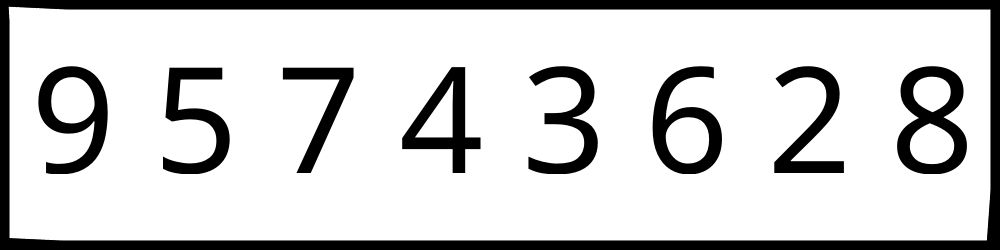
\includegraphics[width=0.4\textwidth]{photos/1.jpg}
    % \caption*{Подпись к фотографии}
\end{figure}

Let's divide our array in 4 equal parts (about the same size). In each quarter, we find every subset sum in $O(2^{n/4})$ or $O(n \cdot 2^{n/4})$ time, it does not matter. After that, we sort subset sums in each quarter in $O(2^{n/4} \log (2^{n/4})) = O(n \cdot 2^{n/4})$ time.

\begin{figure}[htbp]
    \centering
    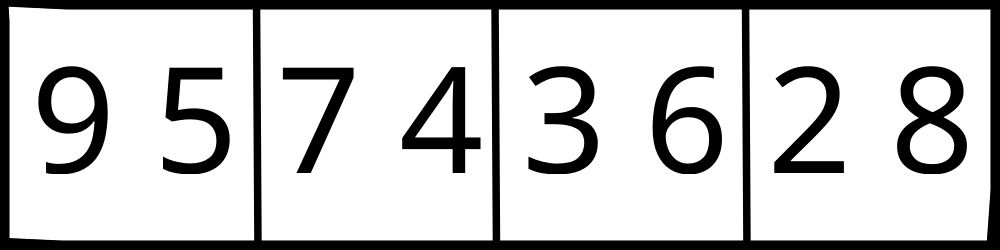
\includegraphics[width=0.4\textwidth]{photos/2.jpg}
    % \caption*{Подпись к фотографии}
\end{figure}

\clearpage

\noindent
\begin{center}
    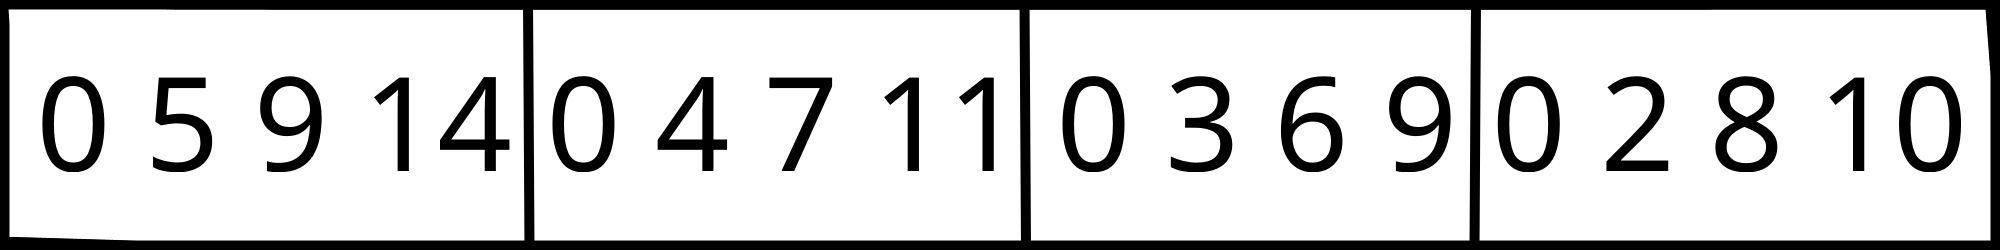
\includegraphics[width=0.8\textwidth]{photos/3.jpg}
\end{center}

After that, we do the following: we take first quarter, combine every element with the minimum in the second quarter (in this situation, it will be just 0) and add to any structure like priority queue, set or heap. We do the same thing with two last quarters but we combine every element from third quarter with the maximum one in the last quarter.

\begin{figure}[htbp]
    \centering
    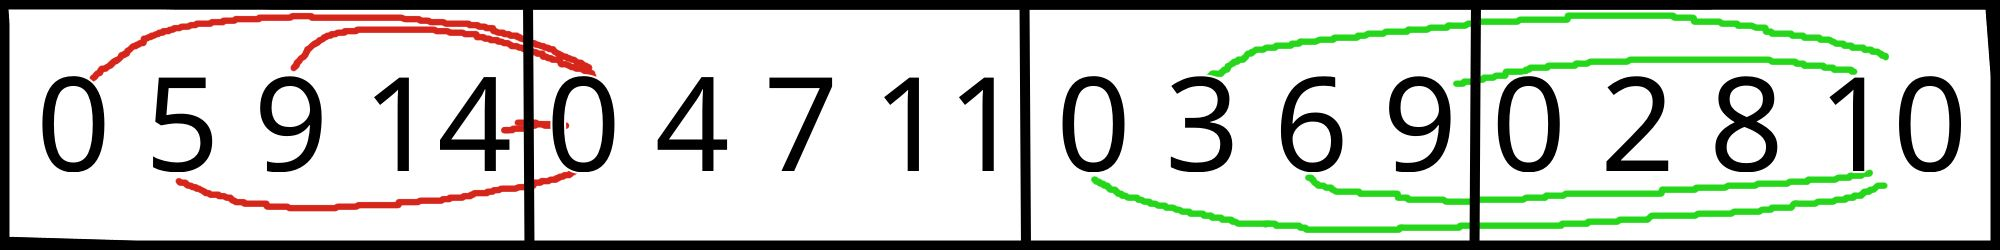
\includegraphics[width=0.8\textwidth]{photos/4.jpg}
    % \caption*{Подпись к фотографии}
\end{figure}

\begin{figure}[htbp]
    \centering
    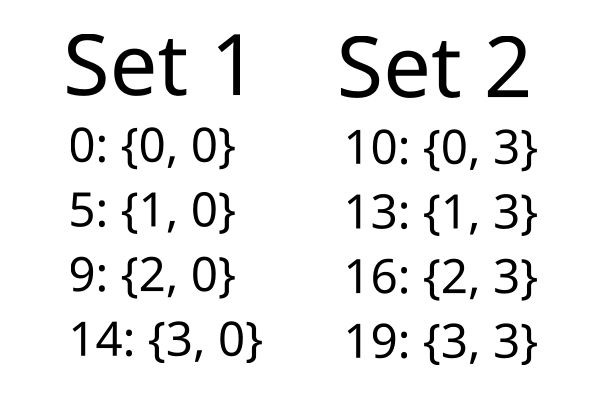
\includegraphics[width=0.4\textwidth]{photos/5.jpg}
    % \caption*{Подпись к фотографии}
\end{figure}

Also, with the sum, we should keep info of both positions in each quarter, we will need it. 

And with this structure, we use a two pointers technique: in the first set, we will go in ascending order with the sum, in the second one - in the descending order. Imagine we take a minimum element in the first set - we want to find a pair in the second one so our sum will be exactly up to $C$: we start by observing the maximum element in the second set so we have $0 + 19 = 19 > 18$, as our sum is greater than $18$ we do the following: we delete pair $\{3, 3\}$ and add pair $\{3, 2\}$. So, every time we are working with a set, we contain a corresponding element in fourth quarter to every element in third quarter by going in descending order in fourth quarter (so that our sums will decrease). New element $17: \{3, 2\}$ will appear. Right now, our sum is $0 + 17 < 18$ and our first pointer moves.

In the first set, we also do the same thing but in ascending order with the elements in second quarter. So we delete $0: \{0, 0\}$ and add $4: \{0, 1\}$. Right now, our sets look like:

\begin{figure}[htbp]
    \centering
    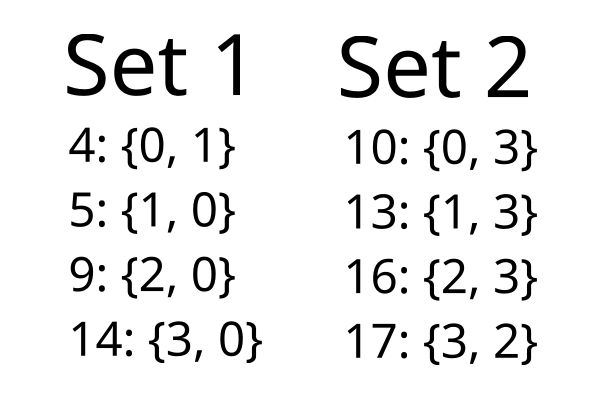
\includegraphics[width=0.4\textwidth]{photos/6.jpg}
    % \caption*{Подпись к фотографии}
\end{figure}

And we continue doing the same two pointers technique unless we find an exact combination that adds up to $C = 18$. For example, we will first encounter it on $5 + 13$.

So, let's count our time and space complexity. As we use two pointers, we already have $O(2^{n/2} \log (2^{n/2})) = O(n \cdot 2^{n/2})$ time complexity so we lost in time a bit (comparing with $O(2^{n/2})$). But space complexity optimized down to $O(2^{n/4})$ as we only need to store vector in each quarter and our sets (or priority queues) use only $O(2^{n/4})$ space so in general we have $O(2^{n/4})$ space complexity.

As a result, we have a $O(n \cdot 2^{n/2})$ time and $O(2^{n/4})$ space solution.

\section{Conclusion}

Some of you might say that this algorithm is worse as it requires more time to be written and loses in time to simple solutions. But this $n$ in $O(n \cdot 2^{n/2})$ does not significantly affect the runtime as it actually is $n/4$ (since sets contain up to $2^{n/4}$ elements) and in real tasks where size of array is bounded mainly with $n \le 40$, $n/4$ does not make this solution super slower. But it gives a cool boost in space complexity.

Hope you enjoyed reading this blog :D

\end{document}